% Tento soubor nahraďte vlastním souborem s přílohami (nadpisy níže jsou pouze pro příklad)

\chapter{Obsah přiloženého paměťového média}
Přiložené médium obsahuje:
    \begin{itemize}
        \item tento soubor ve formátu PDF,
        \item zdrojové kódy (\LaTeX) této práce,
        \item kompletní zdrojové kódy pro sběr dat,
        \item kompletní zdrojové kódy pro extrakci příznaků,
        \item kompletní zdrojové kódy pro trénování klasifikátorů,
        \item manuál k použití.
    \end{itemize}
        

\chapter{Seznam příznaků}
V~této příloze se nachází tabulka~\ref{tab:all_features}, která zobrazuje seznam příznaků seřazených podle vlivu a důležitosti podle SHAP. V~prvním sloupci je samostatná hodnota SHAP, v~dalším je kategorie do které daný příznak spadá, poté i jeho celé jméno, jak je v~kódu a v~posledním sloupci je vysvětlení, co daný příznak znamená.

V~tabulce jsou použity i zkratky, proto zde je výpis těch, které nemusí být na první pohled patrné:
\begin{itemize}
    \item SLD -- doména druhé úrovně,
    \item TLD -- doména první úrovně,
    \item DN -- doménové jméno,
    \item RR -- zdrojový záznam v~DNS (A, AAAA, ...),
    \item SAN -- alternativní názvy subjektů,
    \item AS -- autonomní systém,
    \item NS -- name server,
    \item VPS -- virtuální privátní server.
\end{itemize}
\begin{landscape}
\begin{center}
        \begin{longtable}{|l|l|l|p{10cm}|}
        \caption{Seznam příznaků využitých pro klasifikátory} \label{tab:all_features} \\
    
        \hline 
        \multicolumn{1}{|c|}{\textbf{SHAP}} & 
        \multicolumn{1}{c|}{\textbf{Kategorie}} & 
        \multicolumn{1}{c|}{\textbf{Název příznaku v~kódu}} & 
        \multicolumn{1}{c|}{\textbf{Význam příznaku}} \\ 
        \hline 
        \endfirsthead

        \caption{Seznam příznaků využitých pro klasifikátory} \\
        \hline 
        \multicolumn{1}{|c|}{\textbf{SHAP}} & \multicolumn{1}{c|}{\textbf{Kategorie}} & \multicolumn{1}{c|}{\textbf{Název příznaku v~kódu}} & \multicolumn{1}{c|}{\textbf{Význam příznaku}} \\ \hline 
        \endhead
        
        \hline \hline
        \endfoot    
        
        \hline \hline
        \endlastfoot
        
        1.359 & IP & ip\_as\_address\_entropy & entropie IP prefixů AS \\
        1.357 & RDAP & rdap\_ip\_v4\_count & počet IPv4 adres v~RDAP \\
        1.267 & lexikální & lex\_sub\_count & počet subdomén \\
        0.850 & lexikální & lex\_tld\_abuse\_score & skóre pro nejpoužívanější TLD \\ 
        0.564 & IP & ip\_count & počet IP adres \\
        0.550 & RDAP & rdap\_domain\_age & počet dní od registrace domény \\
        0.549 & lexikální & lex\_tld\_hash & hash TLD \\
        0.505 & IP & ip\_mean\_average\_rtt & průměrná RTT všech pokusů ICMP Echo \\ 
        0.492 & TLS & tls\_expired\_chain & příznak, zda je v~řetězci certifikát s~prošlou platností \\
        0.489 & DNS & dns\_A\_count & počet záznamů A~\\
        0.459 & lexikální & lex\_tld\_len & délka TLD \\
        0.447 & RDAP & rdap\_time\_from\_last\_change & počet dní od poslední změny \\
        0.413 & RDAP & rdap\_registrar\_name\_len & délka jména registrátora \\
        0.410 & RDAP & rdap\_registrar\_name\_hash & hash jména registrátora \\
        0.385 & IP & ip\_entropy & celková entropie všech /16 (/64 pro v6) IP prefixů\\
        0.382 & DNS & dns\_NS\_count & počet záznamů NS \\
        0.359 & TLS & tls\_chain\_len & délka řetězce certifikátu \\
        0.349 & DNS & dns\_ttl\_stdev & směrodatná odchylka TTL v~rámci sady RRset \\
        0.308 & DNS & dns\_zone\_entropy & normalizovaná entropie zóny DN \\
        0.271 & DNS & dns\_zone\_len & počet znaků v~zóně DN \\
        0.270 & IP & ip\_v4\_ratio & poměr IPv4 ke všem IP adresám \\
        0.260 & RDAP & rdap\_registration\_period & rozdíl mezi datem vypršení platnosti a datem registrace \\
        0.223 & RDAP & rdap\_registrar\_name\_entropy & entropie jména registrátora \\
        0.219 & IP & ip\_distinct\_as\_count & počet různých AS \\
        0.191 & DNS & dns\_ttl\_low & pčet sad RR s~TTL $\in [0, 100]$  \\
        0.184 & lexikální & lex\_stdev\_part\_lens & směrodatná odchylka délky částí doménového jména \\
        0.183 & DNS & dns\_ttl\_avg & průměrná hodnota TTL napříč sadami RRs  \\
        &&&\\        
        \multirow{3}{*}{0.181} & \multirow{3}{*}{TLS} & \multirow{3}{*}{tls\_joint\_isoitu\_policy\_crt\_count} & počet certifikátů s~politikou z~Joint ISO ITU-T \\
        & & & \textit{certifikáty s~rozšířením Certificate Policies, které obsahují politiku s~OID z~Joint ISO ITU-T podstromu (2)} \\
        0.173 & RDAP & rdap\_ip\_avg\_admin\_name\_len & průměrná délka jména správce pro IP adresy \\
        0.167 & DNS & dns\_ttl\_distinct\_count & počet různých hodnot TTL v~sadách RRsets \\
        0.160 & DNS & dns\_MX\_count & počet záznamů MX \\
        0.143 & RDAP & rdap\_ip\_avg\_admin\_email\_entropy & průměrná entropie e-mailu správce pro IP adresu \\
        0.134 & DNS & dns\_soa\_retry & SOA retry parametr \\
        0.125 & lexikální & lex\_malware\_pentagram\_matches & počet běžných shod malwarových pentagramů v~DN \\
        0.124 & RDAP & rdap\_domain\_active\_time & min(dnešní datum, expirace) - datum registrace \\
        0.123 & geolokace & geo\_countries\_hash & jedinečný hash pro každou kombinaci zemí  \\
        0.119 & RDAP & rdap\_ip\_shortest\_v4\_prefix\_len & délka nejkratšího prefixu IPv4 \\ 
        0.117 & lexikální & lex\_malware\_bigram\_matches & počet běžných shod malwarových bigramů v~DN \\
        0.115 & RDAP & rdap\_ip\_v6\_count & počet IPv6 adres v~RDAP \\
        0.113 & lexikální & lex\_avg\_part\_len & průměrná délka částí doménového jména \\
        0.112 & DNS & dns\_AAAA\_count & počet záznamů AAAA \\
        0.111 & lexikální & lex\_sub\_hex\_ratio & poměr hexadecimálních symbolů v~subdoménách \\
        0.111 & lexikální & lex\_sld\_norm\_entropy & normalizovaná entropie SLD \\
        0.103 & RDAP & rdap\_ip\_avg\_admin\_name\_entropy & průměrná entropie e-mailu správce pro IP adresu \\
        0.103 & lexikální & lex\_stld\_unique\_char\_count & počet jedinečných znaků v~TLD a SLD \\
        0.103 & lexikální & lex\_malware\_tetragram\_matches & počet běžných shod malwarových tetragramů v~DN \\
        0.097 & TLS & tls\_leaf\_authority\_hash & hash názvu listové certifikační autority \\
        0.095 & lexikální & lex\_sld\_hex\_ratio & poměr hexadecimálních symbolů v~SLD \\
        0.095 & lexikální & lex\_www\_flag & doména začíná na www \\
        0.094 & RDAP & rdap\_ip\_avg\_admin\_email\_len & průměrná délka e-mailu správce pro IP adresy \\
        0.093 & geolokace & geo\_max\_lon & maximální zeměpisná délka míst IP \\
        0.092 & RDAP & rdap\_ip\_longest\_v4\_prefix\_len & délka nejdelšího prefixu IPv4 \\
        0.091 & lexikální & lex\_sld\_vowel\_ratio & poměr samohlásek v~SLD \\  
        0.091 & lexikální & lex\_malware\_trigram\_matches & počet běžných shod malwarových trigramů v~DN \\
        0.090 & TLS & tls\_negotiated\_cipher\_id & identifikátor vyjednané šifry TLS \\
        0.089 & lexikální & lex\_sub\_non\_alphanum\_ratio & poměr podtržítek a pomlček v~subdoménách \\
        0.087 & lexikální & lex\_sub\_vowel\_ratio & poměr samohlásek v~subdoménách \\
        0.086 & lexikální & lex\_sub\_norm\_entropy & normalizovaná entropie subdomén \\
        0.082 & lexikální & lex\_sub\_consonant\_ratio & poměr souhlásek v~subdoménách \\
        0.081 & DNS & dns\_txt\_avg\_entropy & průměrná normalizovaná entropie hodnot TXT RRs \\
        0.081 & DNS & dns\_soa\_refresh & SOA refresh parametr \\
        0.079 & lexikální & lex\_sld\_consonant\_ratio & poměr souhlásek v~SLD \\
        0.079 & DNS & dns\_mx\_avg\_len & průměrný počet znaků v~záznamech MX DN \\
        0.077 & lexikální & lex\_sub\_max\_consonant\_len & nejdelší délka souhláskové sekvence v~subdoménách \\
        0.076 & DNS & dns\_soa\_min\_ttl & SOA minimum TTL \\
        0.075 & DNS & dns\_CNAME\_count & počet záznamů CNAME \\
        0.075 & DNS & dns\_resolved\_record\_types & počet nalezených souborů RR \\ 
        0.069 & RDAP & rdap\_ip\_longest\_v6\_prefix\_len & délka nejdelšího prefixu IPv6 \\
        0.069 & lexikální & lex\_name\_len & délka doménového jména \\    
        0.069 & DNS & dns\_mx\_avg\_entropy & průměrná normalizovaná entropie v~záznamech MX DN \\
        0.064 & DNS & dns\_has\_dnskey & příznak, zda se v~zóně nachází sada DNSKEY RRset \\
        0.064 & TLS & tls\_negotiated\_version\_id & číslo vyjednané verze TLS (TLSv1.x) \\
        0.064 & geolokace & geo\_min\_lat & minimální zeměpisná délka míst IP \\
        0.056 & geolokace & geo\_max\_lat & maximální zeměpisná délka míst IP \\
        0.056 & TLS & tls\_root\_authority\_hash & hash názvu kořenové certifikační autority \\ 
        0.055 & TLS & tls\_total\_extension\_count & celkový počet rozšíření ve všech certifikátech v~řetězci \\
        0.055 & RDAP & rdap\_registrant\_name\_len & délka jména žadatele o~registraci \\
        0.055 & DNS & dns\_soa\_primary\_ns\_entropy & normalizovaná entropie primárního NS DN \\
        0.054 & DNS & dns\_TXT\_count & počet záznamů TXT \\   
        0.054 & lexikální & lex\_consecutive\_chars & nejdelší po sobě jdoucí délka sekvence \\
        0.053 & geolokace & geo\_min\_lon & minimální zeměpisná délka míst IP \\
        0.053 & RDAP & rdap\_ip\_shortest\_v6\_prefix\_len & délka nejkratšího prefixu IPv6 \\
        0.051 & DNS & dns\_soa\_email\_entropy & normalizovaná entropie e-mailu správce DN  \\ 
        0.049 & RDAP & rdap\_registrant\_name\_entropy & entropie názvu žadatele o~registraci \\
        \multirow{2}{*}{0.047} & \multirow{2}{*}{TLS} & \multirow{2}{*}{tls\_critical\_extensions} & celkový počet rozšíření označených jako "kritická" ve všech certifikátech \\
        0.046 & DNS & dns\_soa\_primary\_ns\_len & počet znaků v~DN primárního NS \\    
        0.044 & IP & ip\_asn\_entropy & entropie čísel AS \\
        0.044 & geolokace & geo\_lon\_range & rozsah zeměpisné délky \\
        0.042 & DNS & dns\_ttl\_mid & počet sad RR s~TTL $\in [101, 500]$ \\
        0.042 & geolokace & geo\_centroid\_lon & střední zeměpisná délka míst IP \\ 
        0.042 & lexikální & lex\_sub\_consonant\_count & počet souhlásek v~subdoménách \\ 
        0.041 & lexikální & lex\_shortest\_sub\_len & nejkratší délka subdomény \\
        0.040 & lexikální & lex\_sld\_len & délka SLD \\
        0.039 & lexikální & lex\_sld\_non\_alphanum\_ratio & poměr podtržítek a pomlček v~SLD \\
        0.038 & lexikální & lex\_sld\_digit\_ratio & poměr číslic v~SLD \\
        0.038 & geolokace & geo\_mean\_lon & průměrná zeměpisná délka míst IP \\
        0.038 & lexikální & lex\_sld\_vowel\_count & počet samohlásek v~SLD \\
        0.038 & geolokace & geo\_mean\_lat & střední zeměpisná šířka míst IP \\
        0.037 & DNS & dns\_SOA\_count & počet záznamů SOA \\
        0.036 & DNS & dns\_soa\_expire & parametr vypršení platnosti záznamu SOA \\
        0.036 & lexikální & lex\_sld\_hex\_count & počet hexadecimálních symbolů v~SLD \\
        0.036 & lexikální & lex\_longest\_part\_len & délka nejdelší části názvu domény \\
        0.035 & geolokace & geo\_continent\_hash & jedinečný hash pro každou kombinaci kontinentů \\
        0.035 & lexikální & lex\_sld\_consonant\_count & počet souhlásek v~SLD \\
        0.034 & DNS & dns\_domain\_name\_in\_mx & příznak, zda je některý poštovní server subdoménou DN \\
        0.033 & lexikální & lex\_sub\_digit\_count & počet číslic v~subdoménách \\
        0.032 & lexikální & lex\_sub\_hex\_count & počet hexadecimálních symbolů v~subdoménách \\
        0.032 & geolokace & geo\_lon\_stdev & směrodatná odchylka od zeměpisných délek míst IP \\
        0.031 & DNS & dns\_soa\_primary\_ns\_digit\_count & počet číslic v~primárním NS DN \\
        0.030 & lexikální & lex\_sub\_digit\_ratio & poměr číslic v~subdoménách \\
        0.030 & RDAP & rdap\_admin\_name\_entropy & entropie jména administrativního kontaktu \\
        0.029 & RDAP & rdap\_admin\_email\_entropy & entropie e-mailu administrativního kontaktu \\
        0.029 & DNS & dns\_txt\_external\_verification\_score & počet řetězců pro ověření dodavatele v~RR TXT \\
        0.028 & lexikální & lex\_sub\_vowel\_count & počet samohlásek v~subdoménách \\
        0.028 & DNS & dns\_soa\_email\_len & počet znaků v~e-mailu správce DN \\
        0.027 & geolokace & geo\_countries\_count & počet různých zemí \\
        0.027 & geolokace & geo\_estimated\_area & přibližná poloha \\
        0.026 & geolokace & geo\_centroid\_lat & střední zeměpisná šířka míst IP \\
        0.026 & DNS & dns\_dnssec\_score & bodování DNSSEC \\
        0.025 & TLS & tls\_client\_auth\_crt\_count & počet certifikátů s~"Ověřování webového serveru" \\
        0.024 & TLS & tls\_x509\_anypolicy\_crt\_count & počet certifikátů, které neprosazují žádnou politiku \\
        0.021 & RDAP & rdap\_admin\_name\_len & délka jména administrativního kontaktu \\ 
        0.020 & TLS & tls\_subject\_count & počet SAN v~listovém certifikátu \\
        0.020 & lexikální & lex\_sub\_non\_alphanum\_count & celkový počet pomlček v~subdoménách \\
        0.018 & TLS & tls\_percentage\_crt\_with\_policies & procento certifikátů s~prodloužením platnosti politik \\    
        0.016 & DNS & dns\_soa\_primary\_ns\_level & počet subdomén v~primárním NS DN \\
        0.016 & TLS & tls\_broken\_chain & příznak, pokud existuje certifikát, který nikdy nebyl platný \\
        0.013 & lexikální & lex\_has\_digit & příznak, zda DN obsahuje číslici \\
        0.012 & DNS & dns\_txt\_spf\_exists & příznak, zda je v~TXT RR záznam SPF \\
        0.012 & geolokace & geo\_lat\_range & rozsah zeměpisné šířky \\
        0.010 & TLS & tls\_CA\_certs\_in\_chain\_ratio & poměr certifikátů certifikačních autorit v~řetězci \\
        0.009 & lexikální & lex\_begins\_with\_digit & příznak, pokud jméno začíná číslicí \\
        0.008 & lexikální & lex\_sld\_digit\_count & počet číslic v~SLD \\
        0.008 & lexikální & lex\_sld\_non\_alphanum\_count & počet pomlček v~SLD \\
        \multirow{3}{*}{0.008} & \multirow{3}{*}{TLS} & \multirow{3}{*}{tls\_iso\_policy\_crt\_count} & počet certifikátů s~politikou z~ISO \\
        & & & \textit{certifikáty s~rozšířením Certificate Policies, které obsahují politiku s~OID z~Joint ISO ITU-T podstromu (1)} \\
        0.008 & DNS & dns\_zone\_digit\_count & počet číslic v~zóně DN \\
        0.006 & DNS & dns\_soa\_email\_digit\_count & počet číslic v~e-mailu správce DN  \\
        0.005 & TLS & tls\_server\_auth\_crt\_count & počet certifikátů s~"Ověřování webového serveru" \\
        0.005 & DNS & dns\_zone\_level & počet subdomén v~zóně DN \\
        0.005 & TLS & tls\_with\_policies\_crt\_count & počet certifikátů, které zahrnují rozšíření zásad \\
        0.004 & DNS & dns\_soa\_email\_level & počet subdomén v~e-mailu správce DN \\
        0.004 & TLS & tls\_common\_name\_count & počet obecných názvů v~řetězci \\
        0.003 & RDAP & rdap\_has\_dnssec & příznak, zda doména používá DNSSEC \\
        0.002 & RDAP & rdap\_admin\_email\_len & délka e-mailu administrativního kontaktu \\
        \multirow{2}{*}{0.001} & \multirow{2}{*}{TLS} & \multirow{2}{*}{tls\_is\_self\_signed} & příznak, zda je listový certifikát podepsán vlastním podpisem \\
        0.000 & DNS & dns\_txt\_dkim\_exists & příznak, zda je v~TXT RR záznam DKIM \\
        0.000 & DNS & dns\_txt\_dmarc\_exists & příznak, zda je v~TXT RR záznam DMARC \\ 



        

        
        
        
        
        
        
        
        
            
        
        
        
         
        \end{longtable}
    \end{center}
\end{landscape}
\chapter{Druhy malwaru v~doménách}
Na následujícím obrázku je možné vidět početní zastoupení jednotlivých domén s~určitým typem malwaru. Tato statistika šla získat pouze z~dat z~ThreatFoxu, tudíž nejsou zde zahrnuté veškeré domény z~datové sady.
\begin{landscape}
    \begin{figure}[htbp]
            \caption{Početní zastoupení jednotlivých domén s~určitým malware typem}
            \scalebox{0.37}{
                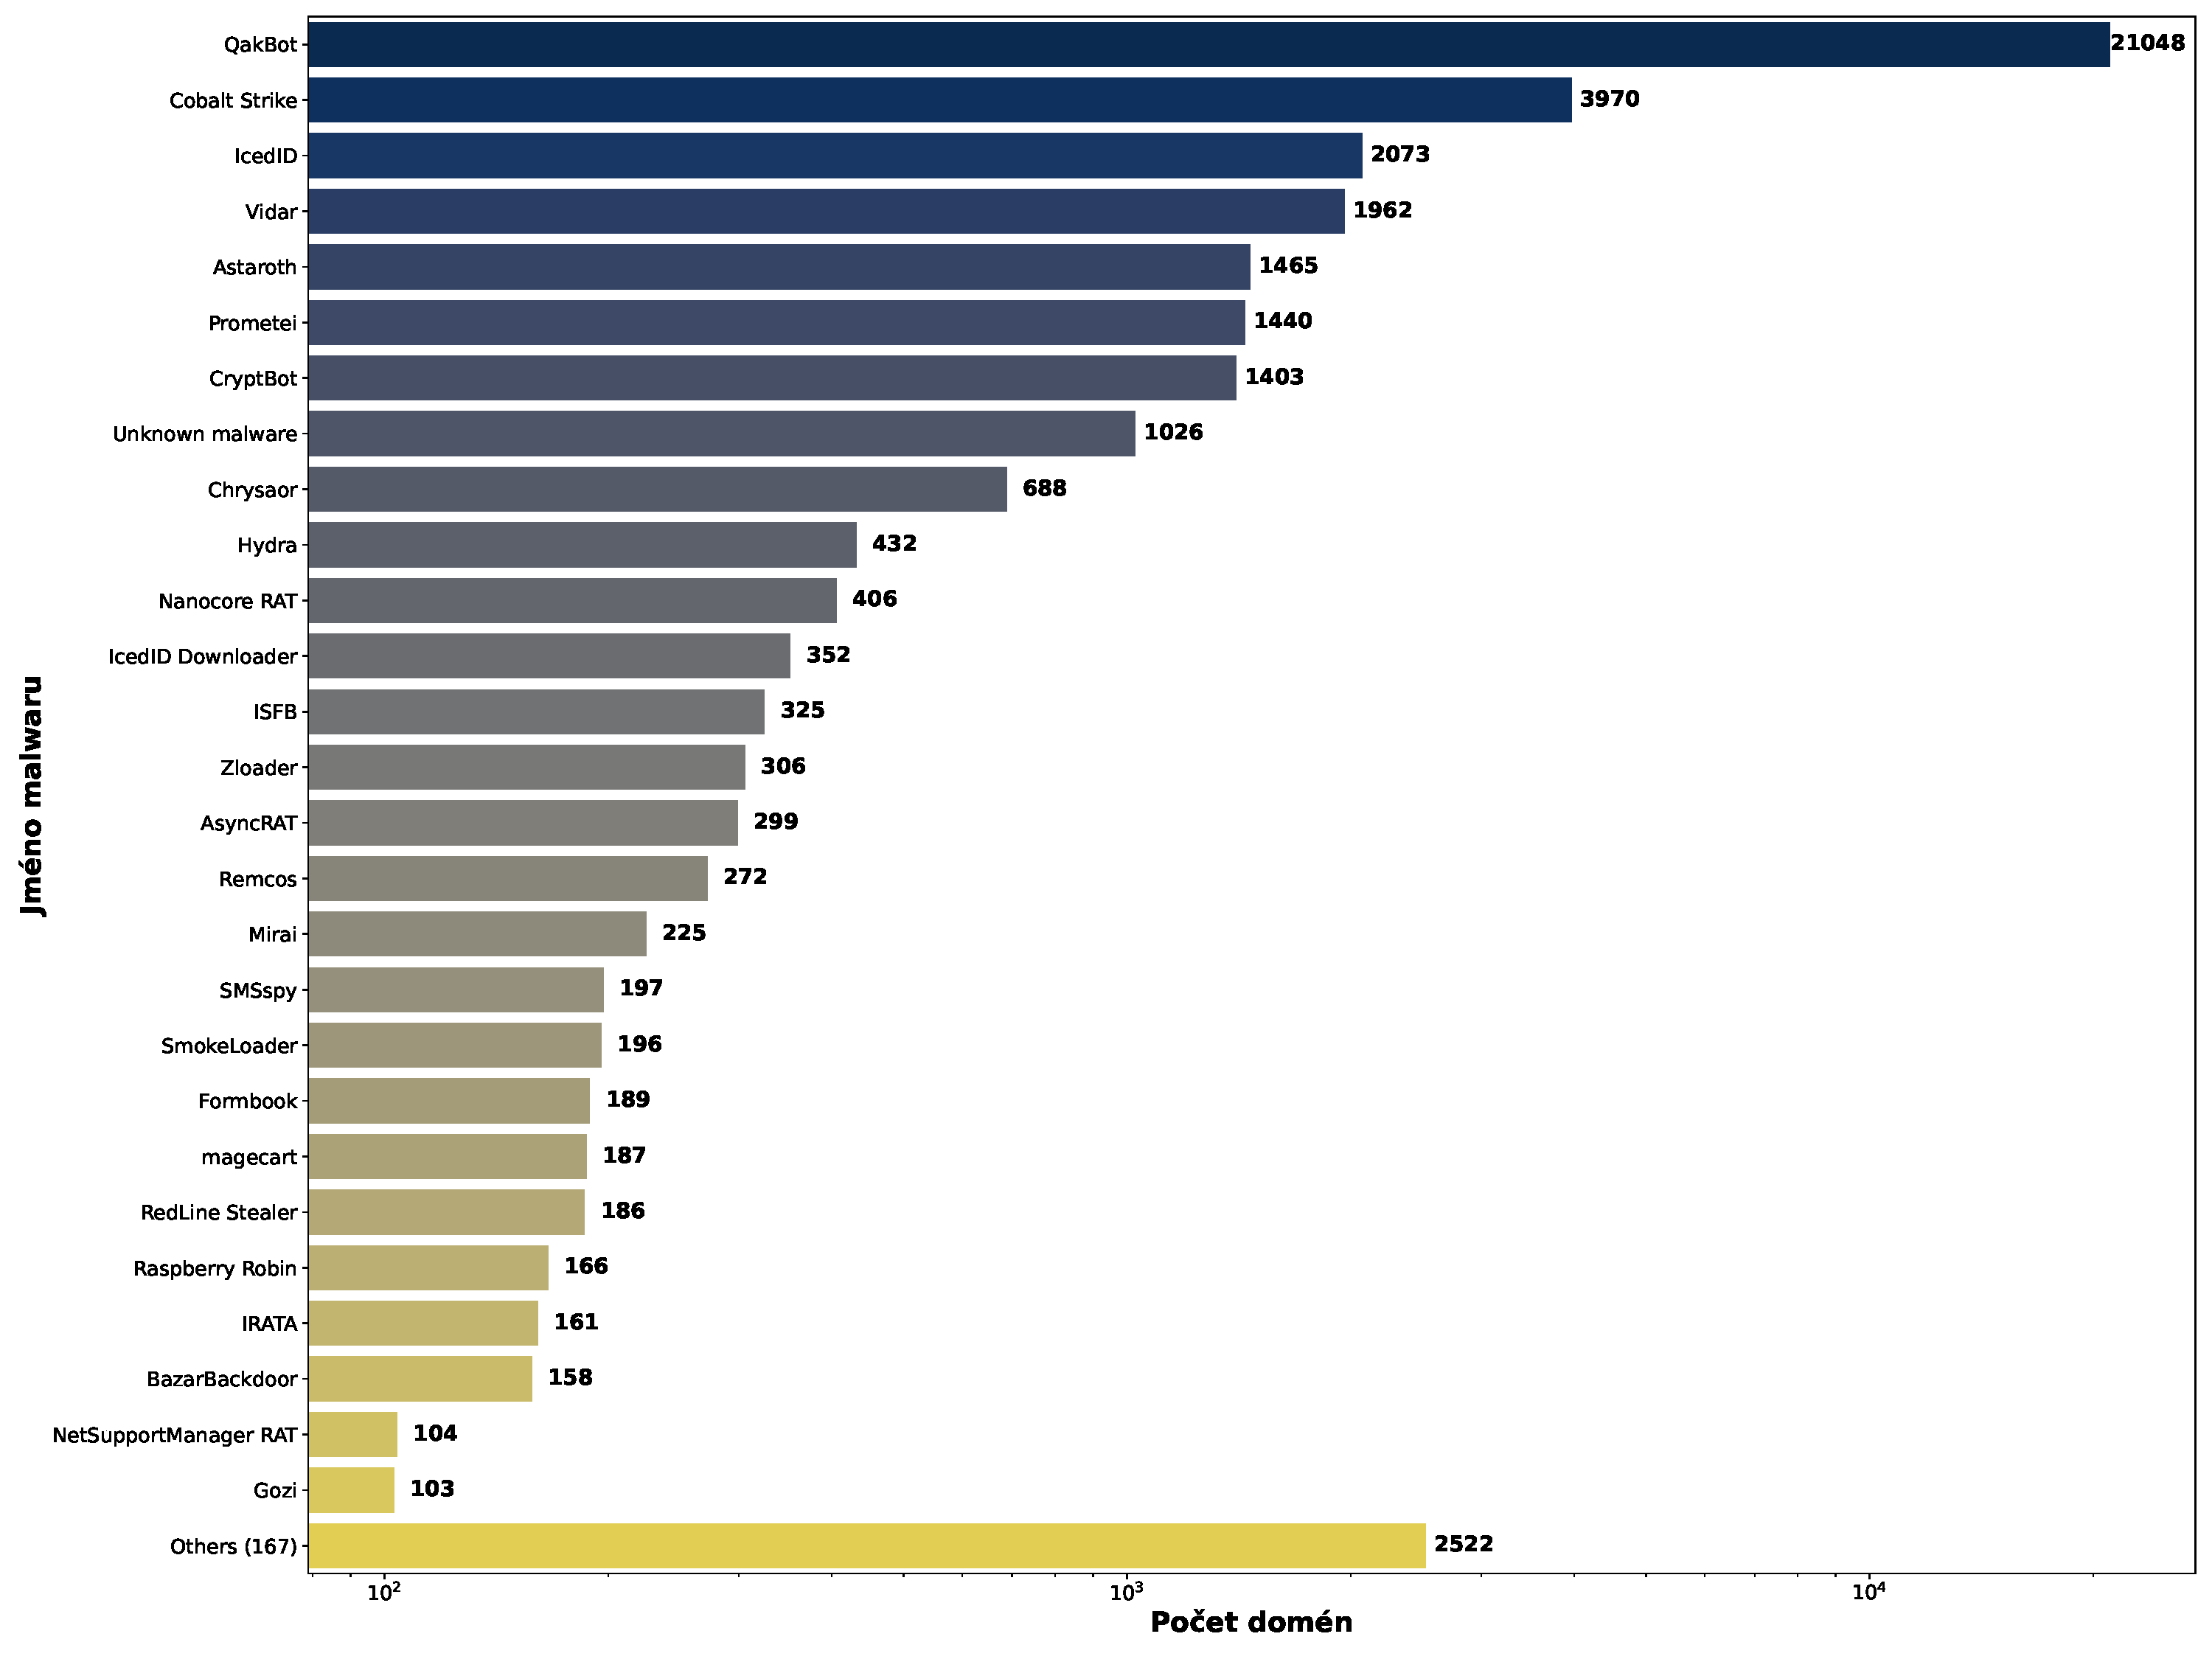
\includegraphics{obrazky-figures/malware_types_barplot.pdf}
            }
            \label{fig:malware_types}
    \end{figure}
\end{landscape}